\documentclass[10pt,a4paper]{article}
\usepackage[utf8]{inputenc}
\usepackage[T1]{fontenc}
\usepackage[margin=0.75in]{geometry}
\usepackage{parskip}
\usepackage{booktabs}
\usepackage{float}
\usepackage{amsmath}
\usepackage{caption}
\usepackage{tikz}
\usetikzlibrary{arrows.meta,positioning,shapes.geometric}
\usepackage{pgfplots}
\pgfplotsset{compat=1.16}
\usepgfplotslibrary{groupplots}

% Signal names with subscripts
\newcommand{\vrefh}{\ensuremath{V_{\mathrm{REFH}}}}
\newcommand{\vrefl}{\ensuremath{V_{\mathrm{REFL}}}}
\newcommand{\vtap}{\ensuremath{V_{\mathrm{TAP}}}}
\newcommand{\vout}{\ensuremath{V_{\mathrm{OUT}}}}
\newcommand{\vdda}{\ensuremath{V_{\mathrm{DDA}}}}
\newcommand{\vddd}{\ensuremath{V_{\mathrm{DDD}}}}
\newcommand{\vssa}{\ensuremath{V_{\mathrm{SS}}}}
\newcommand{\ibias}{\ensuremath{I_{\mathrm{BIAS}}}}
\newcommand{\idda}{\ensuremath{I_{\mathrm{DDA}}}}
\newcommand{\iddd}{\ensuremath{I_{\mathrm{DDD}}}}
\newcommand{\iref}{\ensuremath{I_{\mathrm{REF}}}}
\newcommand{\en}{\ensuremath{\mathrm{EN}}}
\newcommand{\dbus}{\ensuremath{D_5\text{--}D_0}}

\title{\textbf{Buffered 6-Bit Resistor-String DAC in Sky130} \\ \large ICARUS TEAM 4: Flatline}
\author{}
\date{}
\makeatletter\renewcommand{\@maketitle}{\begin{center}{\LARGE \@title \par}\end{center}\vspace{0.5em}}\makeatother

\begin{document}

\maketitle

% ============================================================
\section{Overview}
A voltage-output, 6-bit resistor-string DAC with an integrated unity-gain output buffer, for Chipalooza Challenge \#4 in Sky130. It holds a static voltage between two external references and drives a $100\,\mathrm{k\Omega} \parallel 20\,\mathrm{pF}$ load. Existing Sky130 Chipalooza DACs are AC-only (audio), current-output (IDAC), unbuffered for $\geq 100\,\mathrm{M\Omega}$ loads (8-bit RDAC) or short-term (12-bit CDAC); this block fills the gap for a static, buffered voltage DAC.

% ============================================================
\section{Applications}
\begin{itemize}
    \item Programmable comparator thresholds and trim or calibration voltages
    \item Low-frequency set points routed across the SoC or to a pin
\end{itemize}

% ============================================================
\section{Topology}
\begin{itemize}
    \item \textbf{Resistor string:} 64 matched $\approx 1\,\mathrm{k\Omega}$ poly units between \vrefh{} and \vrefl{}; inherently monotonic
    \item \textbf{Tap selector:} 6-level binary tree of CMOS transmission gates, one level per bit, so no decoder is needed; $\vtap = \vrefl + D\,(\vrefh - \vrefl)/64$, $D = 0\ldots63$
    \item \textbf{Level shifters:} seven cross-coupled shifters convert \dbus{} and \en{} from $1.8\,\mathrm{V}$ logic to complementary $0/3.3\,\mathrm{V}$ switch drives
    \item \textbf{Output buffer:} complementary-input two-stage op-amp at unity gain, Miller-compensated ($60\,\mathrm{pF}$ MIM, $1.5\,\mathrm{k\Omega}$); $1\,\mu\mathrm{A}$ bias mirrored to $10\,\mu\mathrm{A}$ per input pair, $100\,\mu\mathrm{A}$ output
    \item \textbf{Enable:} \en{} low connects the buffer input to \vrefl{}. Codes may change while \en{} is high; brief multi-bit glitches are expected
\end{itemize}

\begin{figure}[H]
\centering
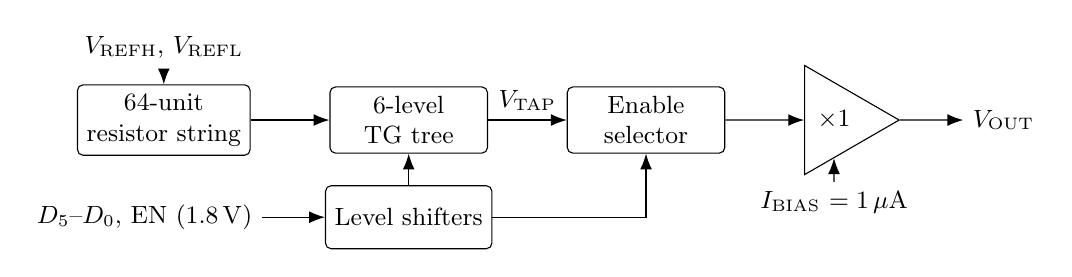
\begin{tikzpicture}[
    blk/.style={draw, rounded corners=2pt, minimum height=8mm, minimum width=20mm, align=center, font=\small},
    arr/.style={-{Latex[length=2mm]}},
    lbl/.style={font=\small}]
  \node[blk] (str) {64-unit\\resistor string};
  \node[blk, right=10mm of str] (tree) {6-level\\TG tree};
  \node[blk, right=10mm of tree] (mux) {Enable\\selector};
  \node[draw, isosceles triangle, isosceles triangle apex angle=60, minimum height=12mm, right=10mm of mux, font=\small] (buf) {$\times 1$};
  \node[blk, below=4mm of tree] (ls) {Level shifters};
  \node[lbl, right=8mm of buf] (out) {\vout};
  \node[lbl, above=2mm of str] (refs) {\vrefh, \vrefl};
  \node[lbl, left=8mm of ls] (dig) {\dbus, \en{} ($1.8\,\mathrm{V}$)};
  \node[lbl, below=3mm of buf] (bias) {\ibias{} $= 1\,\mu\mathrm{A}$};
  \draw[arr] (refs) -- (str);
  \draw[arr] (str) -- (tree);
  \draw[arr] (tree) -- node[above, lbl] {\vtap} (mux);
  \draw[arr] (mux) -- (buf);
  \draw[arr] (buf) -- (out);
  \draw[arr] (dig) -- (ls);
  \draw[arr] (ls) -- (tree);
  \draw[arr] (ls.east) -| (mux.south);
  \draw[arr] (bias) -- (buf);
\end{tikzpicture}
\end{figure}

% ============================================================
\section{Pin List}
\begin{table}[H]
  \centering
  \begin{tabular}{@{}l l l@{}}
    \toprule
    \textbf{Pin} & \textbf{Function} & \textbf{Type} \\
    \midrule
    \dbus       & Data code, $D_5$ = MSB (6 harness control inputs)              & Digital in, $1.8\,\mathrm{V}$ \\
    \en         & Enable; low resets output to \vrefl{} (1 control input)        & Digital in, $1.8\,\mathrm{V}$ \\
    \vrefh      & Upper reference, $3.0\,\mathrm{V}$; sources $\approx 42\,\mu\mathrm{A}$ (shared analog line) & Analog in \\
    \vrefl      & Lower reference, $0.3\,\mathrm{V}$; sinks $\approx 42\,\mu\mathrm{A}$ (shared analog line)   & Analog in \\
    \vtap       & Unbuffered tap; test port and fallback output (shared analog line) & Analog out \\
    \vout       & Buffered DAC output (dedicated pad, requested)                 & Analog out \\
    \ibias      & $1\,\mu\mathrm{A}$ mirrored harness current                     & Bias in \\
    \vdda       & $3.3\,\mathrm{V}$ analog supply (per-slot switch)              & Power \\
    \vddd       & $1.8\,\mathrm{V}$ digital supply                               & Power \\
    \vssa        & Ground                                                         & Power \\
    \bottomrule
  \end{tabular}
\end{table}

Harness resources: 7 of 24 control inputs, 0 status outputs, 3 of 4 shared analog lines, 1 dedicated pad and 1 bias current.

% ============================================================
\section{Target Specifications}
Conditions: $\vrefl = 0.300\,\mathrm{V}$, $\vrefh = 3.000\,\mathrm{V}$, load $100\,\mathrm{k\Omega} \parallel 20\,\mathrm{pF}$ (including pad, package and fixture). $1\,\mathrm{LSB} = 42.1875\,\mathrm{mV}$; errors are referred to the measured references.
\begin{table}[H]
  \centering
  \begin{tabular}{@{}l c c c l@{}}
    \toprule
    \textbf{Parameter} & \textbf{Min} & \textbf{Typ} & \textbf{Max} & \textbf{Unit} \\
    \midrule
    Analog supply \vdda                   & 3.135 & 3.3   & 3.465 & V \\
    Digital supply \vddd                  & 1.71  & 1.8   & 1.89  & V \\
    Temperature                           & $-20$ & 25    & 110   & $^\circ$C \\
    Bias current \ibias                   & 0.8   & 1.0   & 1.2   & $\mu$A \\
    Resolution                            & --    & 6     & --    & bit \\
    Output range (code 0 to 63)           & 0.300 & --    & 2.958 & V \\
    Absolute error, every code            & $-0.5$ & --   & $+0.5$ & LSB \\
    DNL                                   & $-0.5$ & --   & $+0.5$ & LSB \\
    INL (endpoint fit)                    & $-0.5$ & --   & $+0.5$ & LSB \\
    Monotonicity                          & \multicolumn{3}{c}{Guaranteed} & -- \\
    Settling after a code change, $\pm 0.5\,\mathrm{LSB}$ & -- & 10 & 20 & $\mu$s \\
    Reference current \iref               & --    & 42.2  & 60    & $\mu$A \\
    Static analog current \idda{} (excl.\ \iref) & -- & 0.3 & 1.0 & mA \\
    Static digital current \iddd          & --    & 5     & 50    & $\mu$A \\
    \bottomrule
  \end{tabular}
\end{table}

\textbf{Absolute limits:} \vdda{} $0$--$3.6\,\mathrm{V}$; \vddd{} $0$--$1.95\,\mathrm{V}$; references and \vout{} between \vssa{} and \vdda{} with $\vrefl < \vrefh$; digital inputs between \vssa{} and \vddd{}; \ibias{} $\leq 2\,\mu\mathrm{A}$; \vout{} must not be driven or shorted. Sky130 device and pad ratings take precedence.

\textbf{Basis for the values:} the $0.3/3.0\,\mathrm{V}$ references keep the buffer clear of both rails; the $1\,\mathrm{k\Omega}$ unit balances reference current, area and settling; $\pm 0.5\,\mathrm{LSB}$ is a common DAC target and $20\,\mu\mathrm{s}$ suits occasional threshold updates; $20\,\mathrm{pF}$ is our pad, package and fixture estimate; supply tolerance and the $-20\,^\circ$C limit are assumed until harness documentation is published ($110\,^\circ$C follows the Challenge \#4 rules). All will be revisited after layout.

% ============================================================
\section{Verification Plan}
\pgfplotstableread{
code vout errlsb inllsb dnllsb
0 0.300253 5.9929 0.0000 -0.2251
1 0.342431 5.7678 -0.1841 -0.2269
2 0.384609 5.5409 -0.3700 0.2922
3 0.426809 5.8331 -0.0368 0.1376
4 0.469002 5.9707 0.1419 0.1572
5 0.511196 6.1279 0.3401 0.2856
6 0.553396 6.4135 0.6667 0.4284
7 0.595601 6.8419 1.1361 0.5089
8 0.637810 7.3508 1.6860 0.4058
9 0.680015 7.7566 2.1328 0.0822
10 0.722206 7.8388 2.2560 -0.2766
11 0.764382 7.5621 2.0204 -0.4660
12 0.806549 7.0962 1.5955 -0.4575
13 0.848718 6.6387 1.1790 -0.3558
14 0.890890 6.2829 0.8643 -0.2441
15 0.933067 6.0388 0.6611 -0.1669
16 0.975248 5.8719 0.5352 -0.1193
17 1.017430 5.7526 0.4569 -0.0972
18 1.059614 5.6554 0.4007 -0.0831
19 1.101798 5.5723 0.3587 -0.0774
20 1.143982 5.4949 0.3223 -0.0746
21 1.186166 5.4203 0.2887 -0.0718
22 1.228351 5.3485 0.2579 -0.0689
23 1.270535 5.2795 0.2300 -0.0718
24 1.312720 5.2078 0.1992 -0.0689
25 1.354904 5.1388 0.1713 -0.0689
26 1.397089 5.0699 0.1434 -0.0689
27 1.439273 5.0009 0.1155 -0.0718
28 1.481458 4.9292 0.0847 -0.0718
29 1.523642 4.8574 0.0539 -0.0718
30 1.565827 4.7856 0.0232 -0.0718
31 1.608011 4.7138 -0.0076 -0.0746
32 1.650196 4.6392 -0.0412 -0.0746
33 1.692380 4.5646 -0.0747 -0.0746
34 1.734564 4.4900 -0.1083 -0.0774
35 1.776749 4.4126 -0.1447 -0.0802
36 1.818933 4.3324 -0.1840 -0.0859
37 1.861117 4.2465 -0.2289 -0.0916
38 1.903300 4.1549 -0.2794 -0.1029
39 1.945483 4.0521 -0.3412 -0.1255
40 1.987666 3.9266 -0.4257 -0.1763
41 2.029846 3.7503 -0.5610 -0.2894
42 2.072021 3.4609 -0.8093 -0.5437
43 2.114186 2.9173 -1.3120 -0.9709
44 2.156332 1.9464 -2.2418 -1.4502
45 2.198458 0.4962 -3.6510 -1.7757
46 2.240571 -1.2795 -5.3857 -1.7531
47 2.282685 -3.0325 -7.0977 -1.1597
48 2.324823 -4.1922 -8.2164 0.0667
49 2.367013 -4.1255 -8.1087 1.5247
50 2.409265 -2.6008 -6.5429 2.3272
51 2.451551 -0.2735 -4.1746 2.0334
52 2.493824 1.7598 -2.1002 1.2196
53 2.536063 2.9794 -0.8397 0.5527
54 2.578274 3.5321 -0.2459 0.0630
55 2.620464 3.5951 -0.1420 -0.0483
56 2.662650 3.5468 -0.1492 0.0158
57 2.704838 3.5626 -0.0924 0.0045
58 2.747025 3.5672 -0.0468 -0.0124
59 2.789212 3.5547 -0.0183 -0.0237
60 2.831399 3.5310 -0.0010 -0.0350
61 2.873585 3.4960 0.0050 -0.0407
62 2.915771 3.4553 0.0053 -0.0463
63 2.957956 3.4089 0.0000 nan
}\dactt
\begin{itemize}
    \item \textbf{Remaining:} port to Xschem/ngspice and CACE for open-source sign-off; layout with dummies and common-centroid inputs; DRC, LVS and PEX re-simulation over PVT; combined mismatch/PVT; harness switch, pad and \vtap{} line models
    \item \textbf{Silicon:} 64-code sweep over SPI with references on a source/measure unit and a precision DMM (error, DNL, INL, monotonicity); \vtap{} vs.\ \vout{} to separate string and buffer errors; scope settling and glitches ($0 \leftrightarrow 63$, $31 \leftrightarrow 32$); $100\,\mathrm{k\Omega}$ and $1\,\mathrm{M\Omega}$ loads; supply, \ibias{} and temperature extremes
\end{itemize}

\begin{figure}[H]
\centering
\begin{tikzpicture}
\begin{axis}[width=\textwidth, height=7.2cm, xmin=-1, xmax=64, xtick={0,8,...,56,63},
    xlabel={Code $D$}, ylabel={$V_{\mathrm{OUT}}$ (V)}, ymin=0.2, ymax=3.1, ytick={0.3,0.6,...,3.0},
    grid=both, grid style={gray!20}, tick label style={font=\small}, label style={font=\small},
    legend cell align=left, legend style={font=\small, at={(0.02,0.97)}, anchor=north west, fill=white}]
  \addplot[red, dashed, thick, domain=0:63] {0.3 + x*0.0421875};
  \addlegendentry{Ideal line}
  \addplot[blue, densely dotted, thick, domain=0:63] {0.300253 + x*(2.957956-0.300253)/63};
  \addlegendentry{Endpoint line}
  \addplot[only marks, mark=*, mark size=1.3pt] table[x=code, y=vout] {\dactt};
  \addlegendentry{Simulated $V_{\mathrm{OUT}}$}
  \node[font=\small, anchor=south east] at (axis cs:63,0.35) {$1\,\mathrm{LSB} = 42.19\,\mathrm{mV}$};
\end{axis}
\end{tikzpicture}

\vspace{2mm}
\begin{tikzpicture}
\begin{axis}[width=\textwidth, height=7.2cm, xmin=-1, xmax=64, xtick={0,8,...,56,63},
    xlabel={Code $D$}, ylabel={Error ($10^{-3}$ LSB)}, ymin=-10, ymax=10, ytick={-10,-8,...,10},
    grid=both, grid style={gray!20}, tick label style={font=\small}, label style={font=\small},
    legend cell align=left, legend style={font=\small, at={(0.02,0.03)}, anchor=south west, fill=white}]
  \addplot[gray, thick, forget plot] coordinates {(-1,0) (64,0)};
  \addplot[red, thick, mark=*, mark size=1.2pt] table[x=code, y=errlsb] {\dactt};
  \addlegendentry{Accuracy: vs.\ ideal line}
  \addplot[blue, thick, mark=square*, mark size=1.1pt] table[x=code, y=inllsb] {\dactt};
  \addlegendentry{Linearity (INL): vs.\ endpoint line}
  \addplot[green!50!black, thick, mark=triangle*, mark size=1.5pt, unbounded coords=jump] table[x=code, y=dnllsb] {\dactt};
  \addlegendentry{DNL: step from $D$ to $D+1$, minus 1 LSB}
\end{axis}
\end{tikzpicture}

\vspace{1mm}
{\small Accuracy $= +0.0078\,\mathrm{LSB}$ @ $D=10$ \quad Linearity (INL) $= -0.0082\,\mathrm{LSB}$ @ $D=48$ \quad DNL $= +0.0023\,\mathrm{LSB}$ @ $50 \to 51$ \quad Monotonic (min.\ step $42.11\,\mathrm{mV}$)}
\captionsetup{skip=3pt}\caption*{\footnotesize Sky130 pre-layout simulation (pinned BSIM, poly-resistor and MIM models), TT corner, nominal supplies, $100\,\mathrm{k\Omega} \parallel 20\,\mathrm{pF}$ load. Resistors are identical in this run; mismatch is assessed separately.}
\end{figure}

% ============================================================
\section{Deliverables}
\begin{itemize}
    \item Schematics, layout (GDS) and LEF views, testbenches, CACE results and DRC/LVS reports in a public Apache 2.0 repository
    \item Datasheet, bench measurement scripts and published silicon results
\end{itemize}

% ============================================================

\end{document}
